\documentclass[../Main.tex]{subfiles}

\begin{document}

\IfFileExists{NewCommands.tex}       {% Add new commands here.
%
% Use "providecommand" instead of "newcommand" since we
% want to include this file in all subfiles, and if we
% used newcommand it would report the error
% "Command xxx already defined"
%
%
\providecommand{\dmOT}{\Delta m^2_{\rm 12}}
\providecommand{\dmsolar}{\Delta m^2_{\rm solar}}
\providecommand{\dmatm}{\Delta m^2_{\rm atm}}
\providecommand{\dmTT}{\Delta m^2_{\rm atm}}
\providecommand{\dmsq}[1]{\Delta m^{2}_{#1}}
\providecommand{\thatm}{\Delta m^2_{\rm atm}}
\providecommand{\thTT}{\theta_{\rm 23}}
\providecommand{\sinsq}[1]{\sin^{2}(\theta_{#1})}
\providecommand{\sinsqOT}{\sin^{2}(\theta_{\rm 12})}
\providecommand{\sinsqsolar}{\sin^{2}(\theta_{\rm solar})}
\providecommand{\sinsqTT}{\sin^{2}(\theta_{\rm 23})}
\providecommand{\sinsqTwoTT}{\sin^{2}(2\theta_{\rm 23})}
\providecommand{\dcp}{\delta_{\rm CP}}

\providecommand{\gsim}{\gtrsim}
\providecommand{\lsim}{\lesssim}
\providecommand{\Enu}{\rm{E}_\nu}
\providecommand{\Emu}{\rm{E}_\mu}
\providecommand{\Ecasc}{\rm{E}_{\rm casc}}
\providecommand{\Lmu}{\rm{L}_\mu}
\providecommand{\Lnu}{\rm{L}_\nu}
\providecommand{\Thetamu}{\theta_\mu}
\providecommand{\cosThetamu}{\cos{\theta_\mu}}
\providecommand{\cosThetanu}{\cos{\theta_\nu}}
\providecommand{\Thetanu}{\theta_\nu}
\providecommand{\nue}{\nu_{\rm e}}
\providecommand{\numu}{\nu_\mu}
\providecommand{\nutau}{\nu_\tau}

\providecommand{\ket}[1]{|#1\rangle}

\providecommand{\ue}[1]{|U_{e #1}|}
\providecommand{\umu}[1]{|U_{\mu #1}|}
\providecommand{\utau}[1]{|U_{\tau #1}|}
\providecommand{\uesq}[1]{|U_{e #1}|^{2}}
\providecommand{\umusq}[1]{|U_{\mu #1}|^{2}}
\providecommand{\utausq}[1]{|U_{\tau #1}|^{2}}

\providecommand{\Nch}{${\rm N}_{\rm ch}\,$}
\providecommand{\Ndir}{${\rm N}_{\rm dir}\,$}
\providecommand{\Nstr}{${\rm N}_{\rm str}\,$}
\providecommand{\Aeff}{${\rm A}_{\rm eff}\,$}
\providecommand{\Veff}{${\rm V}_{\rm eff}\,$}
\providecommand{\VeffNS}{${\rm V}_{\rm eff}$}

\providecommand{\pe}{$p.e.$ }
}       {}
\IfFileExists{../NewCommands.tex}    {% Add new commands here.
%
% Use "providecommand" instead of "newcommand" since we
% want to include this file in all subfiles, and if we
% used newcommand it would report the error
% "Command xxx already defined"
%
%
\providecommand{\dmOT}{\Delta m^2_{\rm 12}}
\providecommand{\dmsolar}{\Delta m^2_{\rm solar}}
\providecommand{\dmatm}{\Delta m^2_{\rm atm}}
\providecommand{\dmTT}{\Delta m^2_{\rm atm}}
\providecommand{\dmsq}[1]{\Delta m^{2}_{#1}}
\providecommand{\thatm}{\Delta m^2_{\rm atm}}
\providecommand{\thTT}{\theta_{\rm 23}}
\providecommand{\sinsq}[1]{\sin^{2}(\theta_{#1})}
\providecommand{\sinsqOT}{\sin^{2}(\theta_{\rm 12})}
\providecommand{\sinsqsolar}{\sin^{2}(\theta_{\rm solar})}
\providecommand{\sinsqTT}{\sin^{2}(\theta_{\rm 23})}
\providecommand{\sinsqTwoTT}{\sin^{2}(2\theta_{\rm 23})}
\providecommand{\dcp}{\delta_{\rm CP}}

\providecommand{\gsim}{\gtrsim}
\providecommand{\lsim}{\lesssim}
\providecommand{\Enu}{\rm{E}_\nu}
\providecommand{\Emu}{\rm{E}_\mu}
\providecommand{\Ecasc}{\rm{E}_{\rm casc}}
\providecommand{\Lmu}{\rm{L}_\mu}
\providecommand{\Lnu}{\rm{L}_\nu}
\providecommand{\Thetamu}{\theta_\mu}
\providecommand{\cosThetamu}{\cos{\theta_\mu}}
\providecommand{\cosThetanu}{\cos{\theta_\nu}}
\providecommand{\Thetanu}{\theta_\nu}
\providecommand{\nue}{\nu_{\rm e}}
\providecommand{\numu}{\nu_\mu}
\providecommand{\nutau}{\nu_\tau}

\providecommand{\ket}[1]{|#1\rangle}

\providecommand{\ue}[1]{|U_{e #1}|}
\providecommand{\umu}[1]{|U_{\mu #1}|}
\providecommand{\utau}[1]{|U_{\tau #1}|}
\providecommand{\uesq}[1]{|U_{e #1}|^{2}}
\providecommand{\umusq}[1]{|U_{\mu #1}|^{2}}
\providecommand{\utausq}[1]{|U_{\tau #1}|^{2}}

\providecommand{\Nch}{${\rm N}_{\rm ch}\,$}
\providecommand{\Ndir}{${\rm N}_{\rm dir}\,$}
\providecommand{\Nstr}{${\rm N}_{\rm str}\,$}
\providecommand{\Aeff}{${\rm A}_{\rm eff}\,$}
\providecommand{\Veff}{${\rm V}_{\rm eff}\,$}
\providecommand{\VeffNS}{${\rm V}_{\rm eff}$}

\providecommand{\pe}{$p.e.$ }
}    {}
\IfFileExists{../../NewCommands.tex} {% Add new commands here.
%
% Use "providecommand" instead of "newcommand" since we
% want to include this file in all subfiles, and if we
% used newcommand it would report the error
% "Command xxx already defined"
%
%
\providecommand{\dmOT}{\Delta m^2_{\rm 12}}
\providecommand{\dmsolar}{\Delta m^2_{\rm solar}}
\providecommand{\dmatm}{\Delta m^2_{\rm atm}}
\providecommand{\dmTT}{\Delta m^2_{\rm atm}}
\providecommand{\dmsq}[1]{\Delta m^{2}_{#1}}
\providecommand{\thatm}{\Delta m^2_{\rm atm}}
\providecommand{\thTT}{\theta_{\rm 23}}
\providecommand{\sinsq}[1]{\sin^{2}(\theta_{#1})}
\providecommand{\sinsqOT}{\sin^{2}(\theta_{\rm 12})}
\providecommand{\sinsqsolar}{\sin^{2}(\theta_{\rm solar})}
\providecommand{\sinsqTT}{\sin^{2}(\theta_{\rm 23})}
\providecommand{\sinsqTwoTT}{\sin^{2}(2\theta_{\rm 23})}
\providecommand{\dcp}{\delta_{\rm CP}}

\providecommand{\gsim}{\gtrsim}
\providecommand{\lsim}{\lesssim}
\providecommand{\Enu}{\rm{E}_\nu}
\providecommand{\Emu}{\rm{E}_\mu}
\providecommand{\Ecasc}{\rm{E}_{\rm casc}}
\providecommand{\Lmu}{\rm{L}_\mu}
\providecommand{\Lnu}{\rm{L}_\nu}
\providecommand{\Thetamu}{\theta_\mu}
\providecommand{\cosThetamu}{\cos{\theta_\mu}}
\providecommand{\cosThetanu}{\cos{\theta_\nu}}
\providecommand{\Thetanu}{\theta_\nu}
\providecommand{\nue}{\nu_{\rm e}}
\providecommand{\numu}{\nu_\mu}
\providecommand{\nutau}{\nu_\tau}

\providecommand{\ket}[1]{|#1\rangle}

\providecommand{\ue}[1]{|U_{e #1}|}
\providecommand{\umu}[1]{|U_{\mu #1}|}
\providecommand{\utau}[1]{|U_{\tau #1}|}
\providecommand{\uesq}[1]{|U_{e #1}|^{2}}
\providecommand{\umusq}[1]{|U_{\mu #1}|^{2}}
\providecommand{\utausq}[1]{|U_{\tau #1}|^{2}}

\providecommand{\Nch}{${\rm N}_{\rm ch}\,$}
\providecommand{\Ndir}{${\rm N}_{\rm dir}\,$}
\providecommand{\Nstr}{${\rm N}_{\rm str}\,$}
\providecommand{\Aeff}{${\rm A}_{\rm eff}\,$}
\providecommand{\Veff}{${\rm V}_{\rm eff}\,$}
\providecommand{\VeffNS}{${\rm V}_{\rm eff}$}

\providecommand{\pe}{$p.e.$ }
} {}


\graphicspath{{figures/}{Modeling/figures/}}


\section{Backgrounds and Sytematic Uncertainties}\label{sec:BackgroundSystematics}

Here we are going to write some really good words about the
backgrounds, sysematic uncertainties, and the treatment thereof.

Describe the sources of uncertainty, where the knowledge we have comes from, and how we can simulate the different situations. How they are implemented in the fit is discussed in the ``Analysis'' chapter.

\subsection{Cosmic Ray Muons Background}\label{sec:CosmicRayMuons}

\subsection{Bulk Ice Model}\label{sec:BulkIce}

\subsection{Hole Ice}\label{sec:HoleIce}

\subsection{Quantum Efficiency of the Digital Optical Modules}\label{sec:DOMEff}

\subsection{Atmospheric $\nu$ Flux Spectral
  Index}\label{sec:SpectralIndex}

\subsection{Cross-Section}\label{sec:CrossSection}


%\begin{figure}
%\centering
%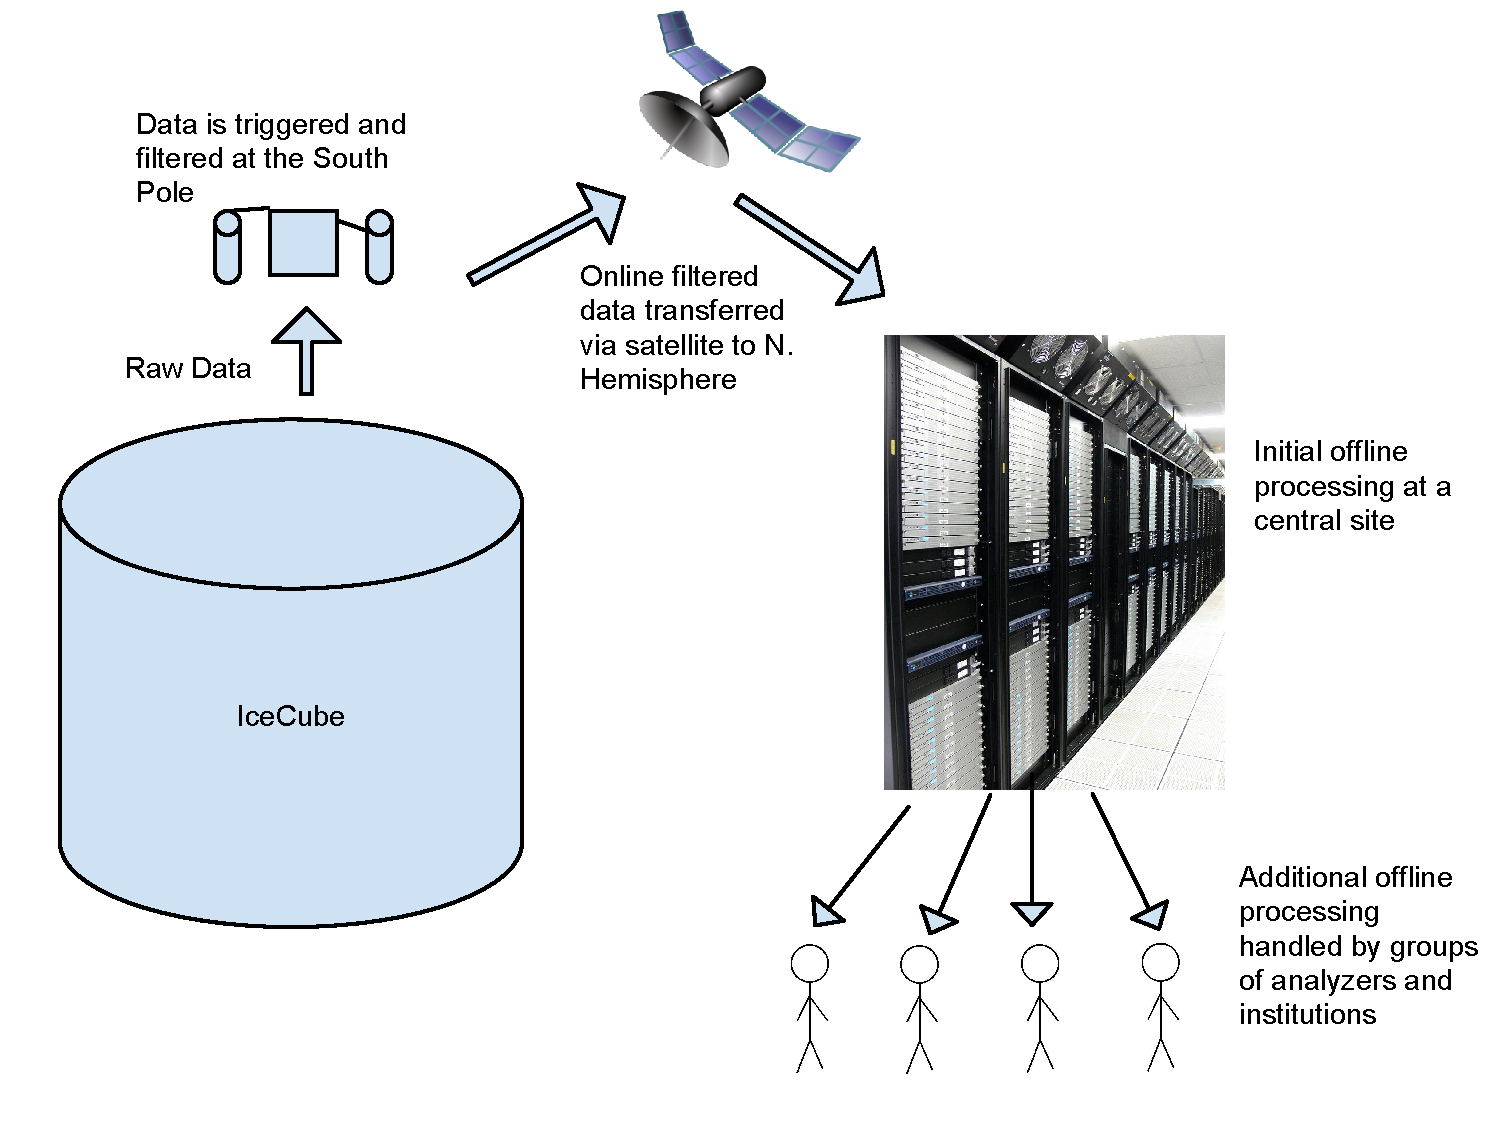
\includegraphics[scale=0.4]{Online_IceCube_data_processing_flow_chart.pdf}
%\caption{\label{fig:DataFlowChart} Should we include, an obviously
%  nicer, flow chart of data collection? More simple? Redundant because
%it'll be in the IceCube Detector paper?}
%\end{figure}

\end{document}
